\chapter{序論}
\label{background}

インターネット上のサービスを提供するサーバー群は、サービスレスポンス時間の短縮や
サービス冗長化のために、複数のデータセンター拠点に展開されている。インターネット上のサービスは複数のコンポーネント
によって構成される。物理的に離れた複数の拠点を用いてサービスを構築するには、他の拠点に設置されたコンポーネントを利用する必要のある場合がある。
物理的に離れた拠点に設置されたコンポーネントを利用すると、拠点間の遅延がコンポーネントのパフォーマンスに大きく影響を与える。
しかし、物理的に離れた拠点間がインターネットを経由して通信する際の経路は、
宛先までの遅延や回線の使用率などを考慮して選択された経路ではないため、遅延が大きくなってしまう
場合がある。

\section{拠点の複数化}
\label{background:multilocation}

近年、インターネット上のサービスはサービスのレスポンス時間を小さく
するためや、自然災害やそれに伴う停電などによるサービスの停止
を避けるため、サービスを複数の拠点に設置している場合が多い。以下で、拠点が複数化する理由の詳細を述べる。

\subsection{レスポンス時間の改善}
\label{background:ml1}

\begin{table}[tb]
	\begin{center}
		\caption{サービスに求められるレスポンス時間}
		\begin{tabular}{|l|l|}
			\hline
				年 & 求められるレスポンス時間 \\
			\hline
				2001年 & 8秒 \\
				2006年 & 4秒 \\
				2009年 & 2秒 \\
			\hline
		\end{tabular}
		\label{table:responsetime}
	\end{center}
\end{table}

サービスの利用者がそのサービスに対しての満足度は、そのサービスのレスポンス時間と関係している。
2001年にZone Research社が行った調査によると、当時、インターネット上のサービス
を利用するにあたり、そのサービスに満足できるレスポンス時間は8秒であった~\cite{zonaresearch}。
レスポンス時間が8秒以上であった場合、そのサービスを利用しなくなってしまうという
結果も出ている。そして、2006年に同じ調査をAkamai社が行った際の結果では、
インターネット上のサービスに求められるレスポンス時間は4秒という結果となった~\cite{akamai4sec}。
更に、同社が2009年に同じ調査を行った際には2秒と更に短くなっていた~\cite{acm:sigops}。これを
表~\ref{table:responsetime}に示した。今後、利用者から求めら
れるレスポンス時間は更に短くなることが予想される。そのため、サービスのレスポンス時間が小さいほど、
利用者は満足すると言える。

近年、サービスを運用するに当たり、サービスの利用者が世界中のどこからでもサービスを満足して利用できるよう、
世界中に設置されたサーバー群の中で最も利用者が満足して
利用できるサーバーからサービスを提供するという手法が用いられることが多い。
この様な手法でサービスを運用しているサービスの例として、Akamai社~\cite{akamai}が提供しているContent Delivery
Network(=CDN)が挙げられる。Akamai社は2010年の時点で61,000台のサーバーを、
1,000以上のネットワーク、世界70カ国以上の拠点に持っている~\cite{acm:sigops}。サービスの利用者が
Akamai社のサービスを利用する際には、このサーバー群の中から、利用者のネットワーク
までの遅延や経路などといった情報をもとに、利用者にとって最も低遅延でサービス
を提供できるサーバーを選択する。これによって利用者は世界中のどこからサービス
を利用しても、満足してそのサービスを利用できるようになる。

このように複数の拠点から同じサービスを提供するという手法は、レスポンス時間を
最小限にする手法として非常に有効である。単一の拠点からサービスを提供した
場合、サービスを提供している拠点とそのサービスの利用者が離れていると
レスポンス時間は長くなる。多くの拠点で同じサービスを提供した場合、利用者にとって一番近い
拠点からサービスを行うことができるので、単一の拠点から提供した
場合と比べるとレスポンス時間は短くなる。レスポンス時間を短くするために、このようなシステムを
運用するこサービスが増えてきているため、サービスを提供するための拠点が増加している。

\subsection{自然災害によるサービス停止の防止}
\label{background:ml2}

自然災害やそれに伴う停電などにより、データセンターが完全に停止してしまう可能性がある。
例えば、2011年3月11日に起きた東日本大震災では、多くのインターネット上のサービスが一時的に停止した。
震災直後は、日本の多くのデータセンターは震災の影響を受けることなく、サービスは継続した。しかし、
その後関東圏で電力不足が生じ、計画停電が実施された。この影響により、
NTTコミュニケーションズ社~\cite{nttcom}が提供している一部法人向けサービスが利用できなくなった~\cite{nttpress}。
慶應義塾大学湘南藤沢キャンパス~\cite{keiosfc}でも計画停電が実施され、多くのサービスを停止
させる必要があった。また、海外でも同様に自然災害によりサービスが停止してしまうという事例がある。
2012年10月、米国東部にハリケーンが上陸し、ニューヨークでは広範囲で浸水に見舞われた。多くの企業が利用しているDataGram社~\cite{datagram}のデータセンター
では、地下が浸水してしまい、その影響により送電網が利用できなくなった。
これにより建物全体が停電し、完全に復旧するのに1週間近くかかった~\cite{datagramdown}。また、Internap社~\cite{internap}
やPEER 1 Hosting社~\cite{peer1}のデータセンターも同様に停電し、全てのサービスが停止した~\cite{nycdown}。

インターネット上のサービスが一時的に利用できなくなると、そのサービスを利用しなくなってしまう
場合がある。2009年に行われた調査によると、有名なオンラインショッピングサイトが1時間利用できなくなった場合、損失は
280万ドル以上になるという~\cite{acm:sigops}。このような損失を防ぐためには、サービスの停止
を防ぐ必要がある。

自然災害や障害によるサービス停止を防ぐために、近年では複数拠点から同じ
サービスの提供をすることや、サービスの複製を行うことが多い。近年では、
インターネット上のサービスの多くが、単一の拠点内で構成される冗長構成だけでなく、
複数の拠点を利用した何重もの冗長構成で構築されている。複数の拠点を利用した冗長構成では、
サービスを提供している拠点の1つが利用できなくなった場合でもサービスの継続が可能である。例えば、
Amazon Web Services社~\cite{aws}が提供しているS3ストレージサービスは、複数の拠点に同じデータを複製している~\cite{awswhite}。
そのため、1つの拠点が利用できなくなった場合でも、他拠点から同じデータを利用することができる。
このような構成で行われるサービスが増えているため、サービスを提供するための拠点が増加している。

\section{遅延が考慮されないインターネットの経路}
\label{background:internetroute}

現在のインターネットの経路は必ずしも遅延が最も小さい経路ではない。インターネットの経路は
Border Gateway Protocol(=BGP)によって学習と選択がされている。BGPでは経路が
最もホップするAutonomous System(=AS)の数が少ないものを優先して経路が選択される。直接経路を交換している(=ピアリング)を
行なっている相手と通信する際には、ピアリングを行なっている拠点を経由する。ピアリングを行なって
いない相手に関してはトランジットを経由する。この仕組では、例えば、通信元と通信先が両方東京に設置
されていたとしても、通信元のネットワークと通信先のネットワークが大阪でピアリングを行なっている場合、
通信は必ず大阪を経由する。このようにBGPを利用した経路選択は、宛先に到達するまでの遅延や
距離、リンクの占有率などを考慮していない。また、BGPにはビジネスの側面がある。例えば、2008年10月30日、
アメリカの大手インターネットプロバイダーであるCogent Communications社~\cite{cogent}とSprint社~\cite{sprint}間でピアリングを行う
にあたっての条件を両者で合意できなくなったため、ピアリングを止めた~\cite{cogentpeering}。これにより、両者のネットワーク間で
通信するためには、非常に遠い経路を通る必要が生じた。このように、BGPを利用した現在のインターネットの経路
では、宛先によっては遅延の大きい経路が選択されてしまう可能性がある。

遅延を削減するためには、他の拠点を一旦経由してから最終的な宛先に到達することでBGPによる
経路よりも小さい遅延で宛先に到達できる場合がある~\cite{netvirt}。MITのHariharan Rahul氏やArthur Berger氏らによる研究~\cite{mittech}では、世界77カ国
からなる1100以上の拠点に設置されたサーバー間の遅延を計測した。その結果、世界中の全経路のうち
約35\%の経路が、他の拠点を経由することによって30\%の遅延削減が可能だ、とされている。特に
通信元と通信先の両方がアジア圏の通信の一部では、他の拠点を経由することにより、50\%以上の遅延削減が可能
である場合もあった。このように、現在のインターネットではインターネットの経路で直接
転送するよりも、他の拠点を経由させることによって、より小さい遅延で通信できる場合がある、ということが
わかる。

\section{拠点の複数化による利点と欠点}
\label{background:ml3}

インターネット上のサービスを複数の拠点で展開することにより、サービスのレスポンス時間の向上や
耐障害性の向上などといった利点を得ることができる。しかし、その一方で、広域にサービスを構成する
コンポーネントが分散することにより生じる遅延により、場合によってはレスポンス時間が低下してしまう可能性
がある。以下で、このような拠点の複数化を行った際に生じる欠点を詳しく述べる。

\subsection{Layer 2ネットワーク拡張技術を用いた複数拠点の運用}
\label{backgound:ml31}

\begin{figure}
	\begin{center}
		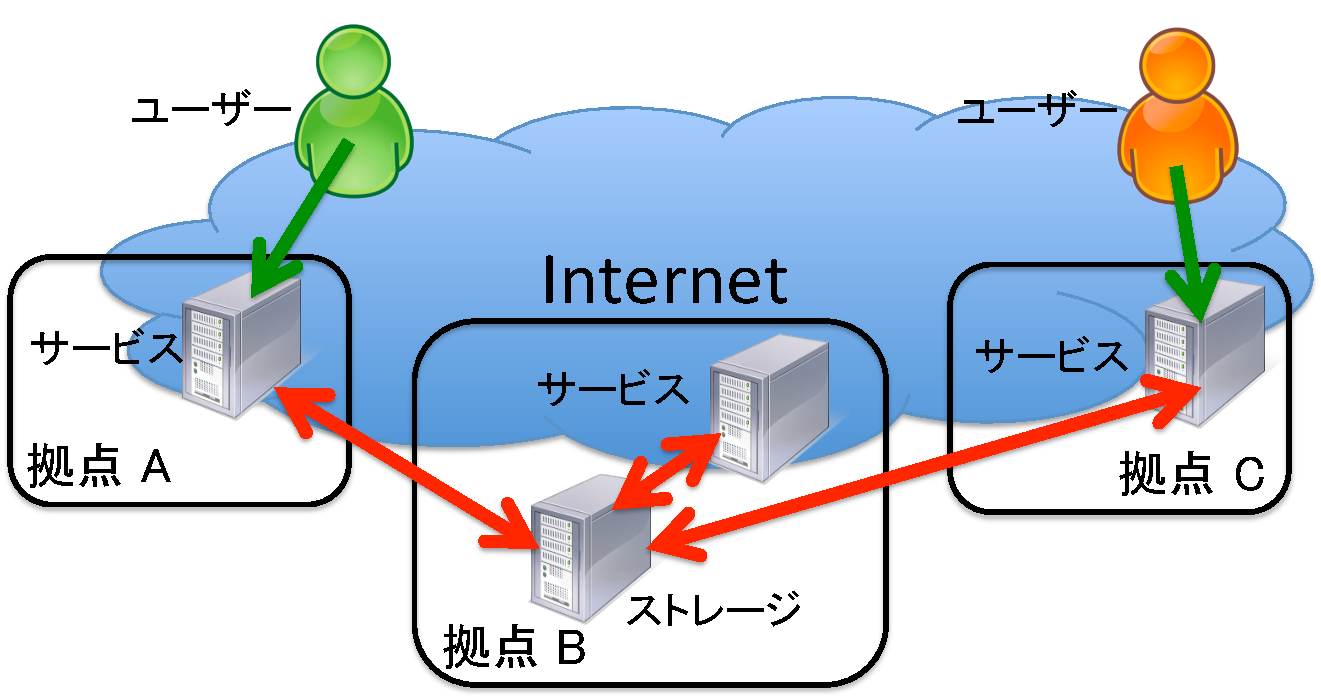
\includegraphics[scale=0.50]{./img/serviceanduser}
		\caption{複数の拠点から提供されるサービス}
		\label{img:mlservice}
	\end{center}
\end{figure}

%%インターネット上のサービスは様々なコンポーネントから構成されている。例えば、オンラインストレージサービス
%%を提供するためには、大きく分けてWebサーバー、ストレージサーバーとデータベースサーバーという3つ
%%のコンポーネントから構成される。Webサーバーは利用者へアップロードやダウンロードなどといったフロントエンド
%%インターフェースを提供する。そして、実際にアップロードされたデータを記憶するストレージサーバー

利用者がサービスを利用するにあたり、利用者はサービスが提供するフロントエンドのインターフェースのみを参照する。
しかし、インターネット上のサービスは、図~\ref{img:mlservice}で示すように、サーバーやストレージ、ネットワークゲートウェイ
などといった複数のコンポーネントから構成されている。フロントエンドのインターフェースの裏では、サービスを動かすために必要となる
ストレージやデータベースなどといった様々なバックエンドのコンポーネントが存在する。例えば、オンラインストレージサービス
は、主に利用者が実際にアップロードやダウンロードなどの操作を行うWebサーバー、実際にアップロードされた
ファイルが記憶されているストレージサーバー、そしてファイルやユーザー情報の管理を行うためのデータベース
サーバーといった3つのコンポーネントから成り立っている。この内、利用者が操作を行う部分はWebサーバーが提供する
フロントエンドインターフェースのみである。残り2つのコンポーネントを利用者は関知しない。このようにインターネット上のサービスは、
利用者が直接関知しない多くのコンポーネントから構成されており、全てのコンポーネントを連動させることによって
サービスが成り立っている。

サービスを運用するにあたり、コンポーネント間には適切なセキュリティーポリシーを適用する必要がある。サービスを構成させるコンポーネントにはインターネットからアクセス
を許可すると危険なコンポーネントがある。このようなコンポーネントの例として、RPC~\cite{rfc:rpc}やSamba~\cite{id:cifs}など既知のセキュリティーホールが非常に多いもの
が挙げられる。また、利用者のパスワードやデータなどが記憶されていて侵入されると被害が大きいコンポーネント
もある。このようなコンポーネントを利用してサービスを構成する際には、コンポーネント間のセキュリティーポリシーを正しく設定
する必要がある。セキュリティーポリシーはコンポーネントによって異なる。インターネットからのアクセスを一切受け付けなくても
良いコンポーネントもあれば、一部の通信のみ受け付ける必要があるコンポーネントもある。このように個々のコンポーネントに対して異なる
セキュリティーポリシーを適用する必要がある場合は、複数のLayer 2ネットワークを用いて、セキュリティーポリシー
の適用を行う。

分散された複数の拠点においてサービスを展開する場合でも、適切にコンポーネント間のセキュリティーポリシーを適用する必要がある。
しかし、複数の拠点においてコンポーネント間のセキュリティーポリシーを適用するために、拠点毎に
コンポーネント間のセキュリティーポリシーを設定するのは、設定が複雑化しサービスを運用するコストが
非常に高くなる、という問題がある。また、インターネットからのアクセスを許可すると危険なコンポーネントを
他の拠点と共有するためには、そのコンポーネントをインターネット上に設置する必要があるため、危険が生じるという問題がある。
これらの問題を防ぐために、Layer 2ネットワーク拡張技術を用いて、Layer 2ネットワークを
全拠点に延長することにより、同じセキュリティーポリシーのもとでコンポーネント間の通信を可能にする。

しかし、広域な環境では1つの拠点内で運用した場合と比べて遅延が非常に大きいため、広域な環境では
コンポーネントのパフォーマンスが著しく低下してしまう場合がある。1つの拠点内でのコンポーネント
間の遅延は、コンポーネント間の距離が物理的に近いため遅延を考慮する必要がない。それに比べ、複数の拠点に
分散されたコンポーネント間の遅延は、コンポーネント間の距離が物理的に離れている上に、インターネットを経由する。
物理的に離れている場合、データを転送するために時間がかかるため遅延が発生する。さらに、
インターネットでは拠点間が通信するために、多くの拠点を経由する。それにより更に遅延が発生する。
また、経由する拠点にトラフィックが集中している場合は、加えて遅延が発生する。そのため、
コンポーネント間の遅延は、1つの拠点内と比べると非常に大きい。
インターネット上のサービスを構成するために利用される技術の多くは1つの拠点内で利用されることが想定されている
ことが多い。そのため、インターネットのような遅延が大きい環境でコンポーネントを利用した場合、
そのコンポーネントのパフォーマンスが著しく低下してしまう場合がある。

\subsection{WIDE Cloudを例にした複数拠点運用における遅延の影響}
\label{wcclatency}

\begin{figure}
	\begin{center}
		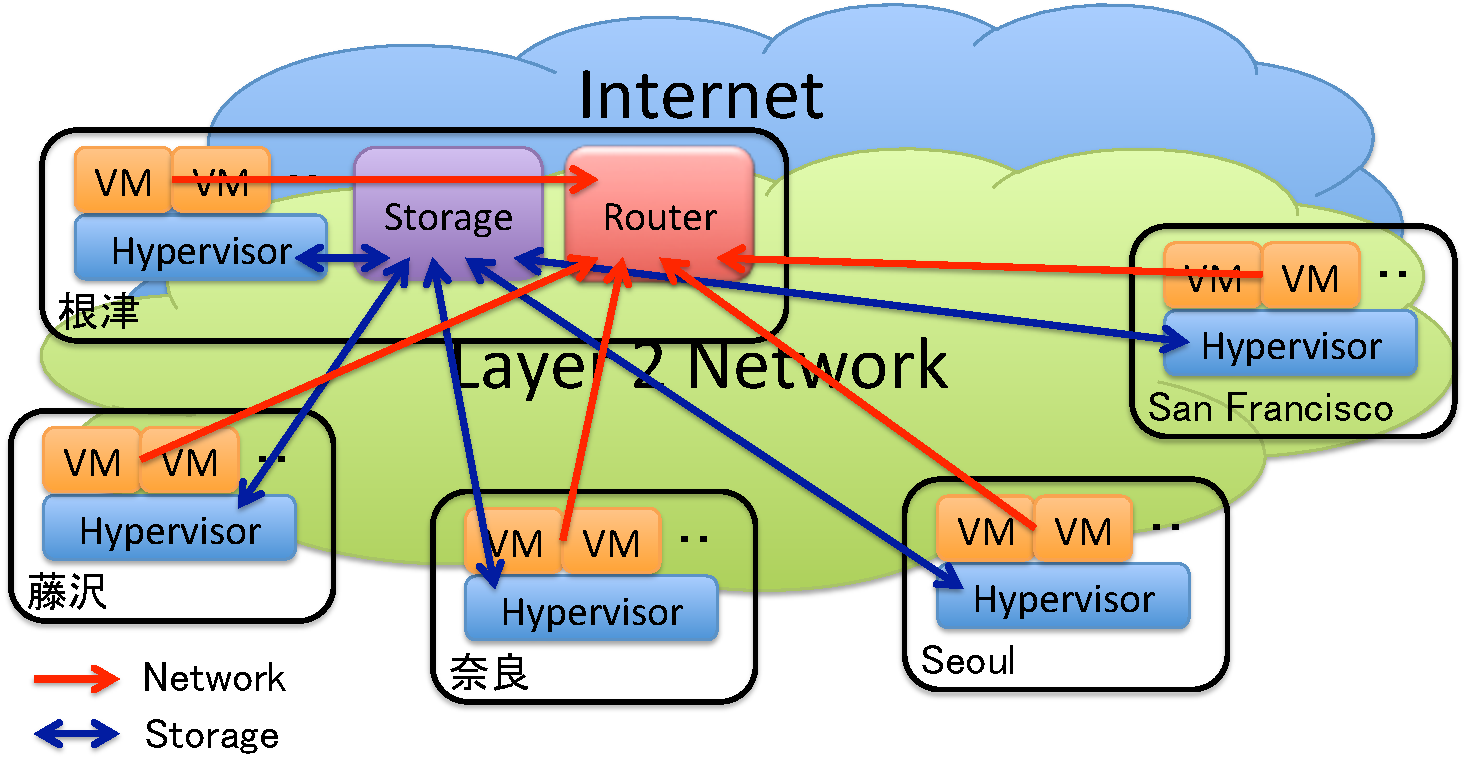
\includegraphics[scale=0.60]{./img/widecloud}
		\caption{WIDE Cloudを構成するコンポーネント}
		\label{img:widecloud}
	\end{center}
\end{figure}

広域環境で運用した際に、パフォーマンスが低下してしまうサービスの例として、WIDE Project~\cite{wideproject}が運用する広域に分散されたIaaS型のクラウド環境
であるWIDE Cloud~\cite{wcc}が挙げられる。WIDE Cloud上に利用者は、仮想マシンを自由に立ち上げることができる。
そして、作成した仮想マシン上で、利用者は任意のサービスを自由に立ち上げることができる。実際、WIDE Cloud上では多種多様なサービスが立ち上げられている。
しかし、これらのサービスのパフォーマンスは、WIDE Cloudのパフォーマンスに影響されている。

WIDE Cloudを構成するコンポーネントとして主に、ハイパーバイザー、ストレージとネットワークゲートウェイの3つのコンポーネントが挙げられる。
各コンポーネントの関係を図~\ref{img:widecloud}に示した。仮想マシン上でサービスを立ち上げるためには、CPU、メモリー、記憶領域とネットワーク
が必要である。この内、CPUとメモリーはハイパーバイザーによって提供される。そして、記憶領域はストレージによって提供される。最後に、
ネットワークはネットワークゲートウェイによって提供される。これらのコンポーネントが連携することにより、仮想マシンが構成されている。

WIDE Cloudを構成するコンポーネントは、離れた複数の拠点に分散されているため、インターネットを経由して利用している。WIDE Cloudの
ハイパーバイザーは日本国内だけでなく、韓国やアメリカなどといった日本国外の拠点にも設置されている。しかし、ストレージとネットワーク
ゲートウェイは日本国内の単一の拠点に設置されている。そのため、多くのハイパーバイザーは遠隔からストレージとネットワークゲートウェイを
利用する。

拠点間でのコンポーネント通信を行うために、WIDE Cloudでは、同一のLayer 2ネットワークを全ての拠点に拡張している。Layer 2ネットワーク
の拡張には、広域Layer 2ネットワークとLayer 2ネットワーク拡張技術を利用している。各拠点に設置されたハイパーバイザーはインターネット上
に拡張されたLayer 2ネットワークを経由して、ストレージとネットワークゲートウェイを利用している。

WIDE Cloud上で動作する仮想マシンのパフォーマンス低下の原因は、ストレージと
ネットワークゲートウェイのパフォーマンス低下である。WIDE Cloudの多くのハイパーバイザーはストレージとネットワークゲートウェイ
をインターネット経由で利用する。ストレージとネットワークゲートウェイのパフォーマンスは遅延によって、パフォーマンスが著しく
低下する。ストレージまでの遅延は仮想マシンのディスクパフォーマンスに影響する。
ストレージをハイパーバイザーから利用するために、WIDE CloudではNFSv3~\cite{rfc:nfsv3}を利用している。しかし、
既存の研究によると、iSCSI~\cite{rfc:iscsi}とNFSv3は遅延が大きくなるに連れ、パフォーマンスが低下する~\cite{usenix:nfsperformance}。
ストレージのパフォーマンスが低下すると、仮想マシンのディスクパフォーマンス
が低下するため、仮想マシンのパフォーマンスが低下する。また、ネットワークゲートウェイまでの遅延は、仮想マシンのネットワークパフォーマンス
に影響する。仮想マシンがインターネットと通信するためには、必ずネットワークゲートウェイを経由する。
そのため、ネットワークゲートウェイまでの遅延が大きいほど、仮想マシンのネットワークパフォーマンスが
低下する。このような仮想マシンのパフォーマンス低下は、コンポーネント間の遅延が小さいほど、パフォーマンス
に与える影響が小さい。

コンポーネント間の遅延は、Layer 2ネットワーク拡張技術がイーサネットフレームを転送する際に、拠点間の遅延を考慮する
ことによって小さくすることができる。WIDE Cloudでは、広域Layer 2ネットワークとLayer 2ネットワーク拡張技術を用いて、
全拠点に同一のLayer 2ネットワークを拡張している。この2つの技術によって構築されたLayer 2ネットワークのトポロジーは
木構造のトポロジーのため、一部拠点間の遅延が不必要に大きくなっている。また、現在のインターネットには~\ref{background:internetroute}節で説明したような、
直接宛先に転送するよりも、他の拠点を経由して転送するほうが、遅延が小さくなるような経路が存在する。Layer 2ネットワーク
を拡張する際に、Layer 2ネットワークを拡張する技術が遅延を考慮してイーサネットフレームを転送することにより、
コンポーネント間の遅延が小さくなるため、遅延が仮想マシンのパフォーマンスに与える影響を小さくすることができる。

\section{本研究の位置付け}
\label{background:thisresearch}

%現在のインターネット上のサービスの多くは、~\ref{background:multilocation}節で説明したように、レスポンス時間
%を小さくするためや障害によるサービス停止を防ぐために、複数の拠点を利用して運用されている。複数の拠点を利用して
%サービスを構築する際に、サービスを構成するコンポーネントを拠点間で利用する必要がある場合がある。

本研究では、インターネット上に分散された複数の拠点に同一のLayer 2ネットワークを拡張した際に、拡張されたLayer 2ネットワーク上で
動作するサービスの遅延によるパフォーマンス低下を小さくすることを目的とする。これを実現するために、Layer 2ネットワーク拡張技術が
イーサネットフレームを転送する際に、遅延の最も小さい経路で転送することを可能にする。WIDE Cloudのように、サービスを構成するコンポーネント
が複数の拠点に分散しているような構成では、コンポーネント間の遅延が、サービスのパフォーマンスに影響する。
遅延が小さいほど、サービスのパフォーマンスは向上する。しかし、既存のLayer 2ネットワーク拡張技術では、
イーサネットフレームを転送する際に、遅延が最も小さい経路で転送されない。そのため、サービスの
パフォーマンスが低下してしまっている。本研究では、拠点間の遅延を計測し、イーサネットフレーム
を遅延が最も小さくなる経路で転送するLayer 2ネットワーク拡張技術を提案する。これにより、
WIDE Cloudのように複数の拠点を用いて構築されたサービスのパフォーマンスを従来より向上させることができる。


\section{本論文の構成}

本論文の構成を以下に示す。第~\ref{rw}章では、既存のLayer 2ネットワーク拡張技術について整理し、
分散した複数の拠点にLayer 2ネットワークを拡張する際に求められるLayer 2ネットワーク拡張技術を示す。
第~\ref{solv}章では、第~\ref{rw}の内容をふまえた上で実現すべき機能要件について整理し、本研究で
提案する手法について述べる。また、提案する手法の実装についても述べる。第~\ref{experiment}章では、
行った実験とその実験から得られた評価結果を示す。そして、第~\ref{conclusion}で、本研究のまとめ
と今後の展望を述べる。

%%% Local Variables:
%%% mode: japanese-latex
%%% TeX-master: "../yummy_bthesis"
%%% End:
